% Created by tikzDevice version 0.6.1 on 2011-08-02 12:45:25
% !TEX encoding = UTF-8 Unicode
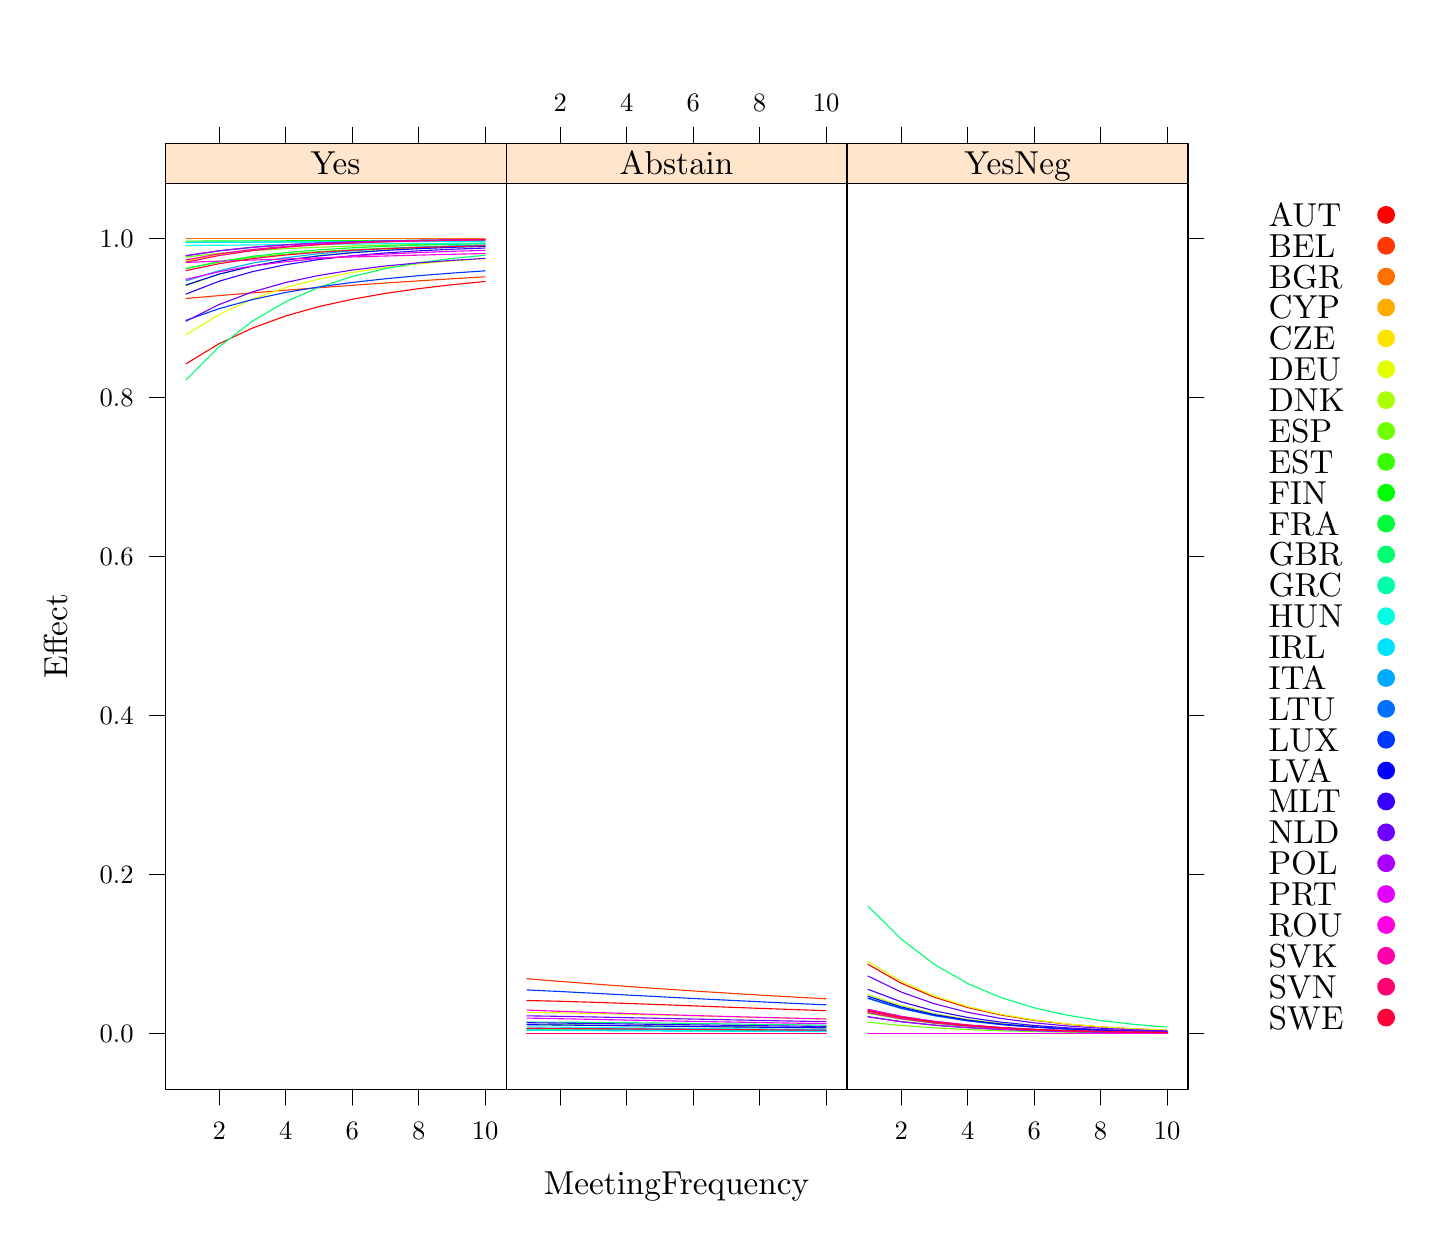
\begin{tikzpicture}[x=1pt,y=1pt]
\definecolor[named]{drawColor}{rgb}{0.00,0.00,0.00}
\definecolor[named]{fillColor}{rgb}{1.00,1.00,1.00}
\fill[color=fillColor,] (0,0) rectangle (505.89,433.62);
\begin{scope}
\path[clip] (  0.00,  0.00) rectangle (505.89,433.62);
\definecolor[named]{fillColor}{rgb}{0.00,0.00,0.00}
\end{scope}
\begin{scope}
\path[clip] (  0.00,  0.00) rectangle (505.89,433.62);
\definecolor[named]{fillColor}{rgb}{0.00,0.00,0.00}

\draw[fill opacity=0.00,draw opacity=0.00,] (  0.00,  0.00) rectangle (505.89,433.62);
\end{scope}
\begin{scope}
\path[clip] (  0.00,  0.00) rectangle (505.89,433.62);
\definecolor[named]{fillColor}{rgb}{0.00,0.00,0.00}
\end{scope}
\begin{scope}
\path[clip] (  0.00,  0.00) rectangle (505.89,433.62);
\definecolor[named]{fillColor}{rgb}{0.00,0.00,0.00}
\definecolor[named]{drawColor}{rgb}{0.00,0.00,0.00}

\node[color=drawColor,anchor=base,inner sep=0pt, outer sep=0pt, scale=  1.20] at (234.47, 12.04) {MeetingFrequency%
};
\end{scope}
\begin{scope}
\path[clip] (  0.00,  0.00) rectangle (505.89,433.62);
\definecolor[named]{fillColor}{rgb}{0.00,0.00,0.00}
\definecolor[named]{drawColor}{rgb}{0.00,0.00,0.00}

\node[rotate= 90.00,color=drawColor,anchor=base,inner sep=0pt, outer sep=0pt, scale=  1.20] at ( 14.29,213.72) {Effect%
};
\end{scope}
\begin{scope}
\path[clip] (  0.00,  0.00) rectangle (505.89,433.62);
\definecolor[named]{fillColor}{rgb}{0.00,0.00,0.00}
\end{scope}
\begin{scope}
\path[clip] (  0.00,  0.00) rectangle (505.89,433.62);
\definecolor[named]{fillColor}{rgb}{0.00,0.00,0.00}
\end{scope}
\begin{scope}
\path[clip] (  0.00,  0.00) rectangle (505.89,433.62);
\definecolor[named]{fillColor}{rgb}{0.00,0.00,0.00}
\end{scope}
\begin{scope}
\path[clip] ( 49.65, 50.02) rectangle (172.86,377.42);
\definecolor[named]{fillColor}{rgb}{0.00,0.00,0.00}
\end{scope}
\begin{scope}
\path[clip] (  0.00,  0.00) rectangle (505.89,433.62);
\definecolor[named]{fillColor}{rgb}{0.00,0.00,0.00}
\end{scope}
\begin{scope}
\path[clip] (  0.00,  0.00) rectangle (505.89,433.62);
\definecolor[named]{fillColor}{rgb}{0.00,0.00,0.00}
\definecolor[named]{drawColor}{rgb}{0.00,0.00,0.00}

\draw[color=drawColor,line cap=round,line join=round,fill opacity=0.00,] ( 69.22,391.87) -- ( 69.22,397.56);

\draw[color=drawColor,line cap=round,line join=round,fill opacity=0.00,] ( 93.24,391.87) -- ( 93.24,397.56);

\draw[color=drawColor,line cap=round,line join=round,fill opacity=0.00,] (117.26,391.87) -- (117.26,397.56);

\draw[color=drawColor,line cap=round,line join=round,fill opacity=0.00,] (141.28,391.87) -- (141.28,397.56);

\draw[color=drawColor,line cap=round,line join=round,fill opacity=0.00,] (165.29,391.87) -- (165.29,397.56);
\end{scope}
\begin{scope}
\path[clip] (  0.00,  0.00) rectangle (505.89,433.62);
\definecolor[named]{fillColor}{rgb}{0.00,0.00,0.00}
\end{scope}
\begin{scope}
\path[clip] (  0.00,  0.00) rectangle (505.89,433.62);
\definecolor[named]{fillColor}{rgb}{0.00,0.00,0.00}
\definecolor[named]{drawColor}{rgb}{0.00,0.00,0.00}

\draw[color=drawColor,line cap=round,line join=round,fill opacity=0.00,] ( 49.65, 70.12) -- ( 43.95, 70.12);

\draw[color=drawColor,line cap=round,line join=round,fill opacity=0.00,] ( 49.65,127.56) -- ( 43.95,127.56);

\draw[color=drawColor,line cap=round,line join=round,fill opacity=0.00,] ( 49.65,185.00) -- ( 43.95,185.00);

\draw[color=drawColor,line cap=round,line join=round,fill opacity=0.00,] ( 49.65,242.43) -- ( 43.95,242.43);

\draw[color=drawColor,line cap=round,line join=round,fill opacity=0.00,] ( 49.65,299.87) -- ( 43.95,299.87);

\draw[color=drawColor,line cap=round,line join=round,fill opacity=0.00,] ( 49.65,357.31) -- ( 43.95,357.31);

\node[color=drawColor,anchor=base east,inner sep=0pt, outer sep=0pt, scale=  0.96] at ( 38.26, 66.81) {0.0%
};

\node[color=drawColor,anchor=base east,inner sep=0pt, outer sep=0pt, scale=  0.96] at ( 38.26,124.25) {0.2%
};

\node[color=drawColor,anchor=base east,inner sep=0pt, outer sep=0pt, scale=  0.96] at ( 38.26,181.69) {0.4%
};

\node[color=drawColor,anchor=base east,inner sep=0pt, outer sep=0pt, scale=  0.96] at ( 38.26,239.13) {0.6%
};

\node[color=drawColor,anchor=base east,inner sep=0pt, outer sep=0pt, scale=  0.96] at ( 38.26,296.57) {0.8%
};

\node[color=drawColor,anchor=base east,inner sep=0pt, outer sep=0pt, scale=  0.96] at ( 38.26,354.01) {1.0%
};
\end{scope}
\begin{scope}
\path[clip] (  0.00,  0.00) rectangle (505.89,433.62);
\definecolor[named]{fillColor}{rgb}{0.00,0.00,0.00}
\end{scope}
\begin{scope}
\path[clip] (  0.00,  0.00) rectangle (505.89,433.62);
\definecolor[named]{fillColor}{rgb}{0.00,0.00,0.00}
\definecolor[named]{drawColor}{rgb}{0.00,0.00,0.00}

\draw[color=drawColor,line cap=round,line join=round,fill opacity=0.00,] ( 69.22, 50.02) -- ( 69.22, 44.32);

\draw[color=drawColor,line cap=round,line join=round,fill opacity=0.00,] ( 93.24, 50.02) -- ( 93.24, 44.32);

\draw[color=drawColor,line cap=round,line join=round,fill opacity=0.00,] (117.26, 50.02) -- (117.26, 44.32);

\draw[color=drawColor,line cap=round,line join=round,fill opacity=0.00,] (141.28, 50.02) -- (141.28, 44.32);

\draw[color=drawColor,line cap=round,line join=round,fill opacity=0.00,] (165.29, 50.02) -- (165.29, 44.32);

\node[color=drawColor,anchor=base,inner sep=0pt, outer sep=0pt, scale=  0.96] at ( 69.22, 32.02) {2%
};

\node[color=drawColor,anchor=base,inner sep=0pt, outer sep=0pt, scale=  0.96] at ( 93.24, 32.02) {4%
};

\node[color=drawColor,anchor=base,inner sep=0pt, outer sep=0pt, scale=  0.96] at (117.26, 32.02) {6%
};

\node[color=drawColor,anchor=base,inner sep=0pt, outer sep=0pt, scale=  0.96] at (141.28, 32.02) {8%
};

\node[color=drawColor,anchor=base,inner sep=0pt, outer sep=0pt, scale=  0.96] at (165.29, 32.02) {10%
};
\end{scope}
\begin{scope}
\path[clip] (  0.00,  0.00) rectangle (505.89,433.62);
\definecolor[named]{fillColor}{rgb}{0.00,0.00,0.00}
\end{scope}
\begin{scope}
\path[clip] ( 49.65, 50.02) rectangle (172.86,377.42);
\definecolor[named]{fillColor}{rgb}{0.00,0.00,0.00}
\definecolor[named]{drawColor}{rgb}{1.00,0.00,0.00}

\draw[color=drawColor,line cap=round,line join=round,fill opacity=0.00,] ( 57.21,312.15) --
	( 69.22,319.44) --
	( 81.23,325.08) --
	( 93.24,329.44) --
	(105.25,332.83) --
	(117.26,335.48) --
	(129.27,337.60) --
	(141.28,339.31) --
	(153.28,340.72) --
	(165.29,341.91);
\definecolor[named]{drawColor}{rgb}{1.00,0.22,0.00}

\draw[color=drawColor,line cap=round,line join=round,fill opacity=0.00,] ( 57.21,335.76) --
	( 69.22,336.80) --
	( 81.23,337.79) --
	( 93.24,338.74) --
	(105.25,339.65) --
	(117.26,340.52) --
	(129.27,341.34) --
	(141.28,342.13) --
	(153.28,342.88) --
	(165.29,343.59);
\definecolor[named]{drawColor}{rgb}{1.00,0.44,0.00}

\draw[color=drawColor,line cap=round,line join=round,fill opacity=0.00,] ( 57.21,357.31) --
	( 69.22,357.31) --
	( 81.23,357.31) --
	( 93.24,357.31) --
	(105.25,357.31) --
	(117.26,357.31) --
	(129.27,357.31) --
	(141.28,357.31) --
	(153.28,357.31) --
	(165.29,357.31);
\definecolor[named]{drawColor}{rgb}{1.00,0.67,0.00}

\draw[color=drawColor,line cap=round,line join=round,fill opacity=0.00,] ( 57.21,351.26) --
	( 69.22,353.01) --
	( 81.23,354.27) --
	( 93.24,355.16) --
	(105.25,355.79) --
	(117.26,356.23) --
	(129.27,356.55) --
	(141.28,356.77) --
	(153.28,356.93) --
	(165.29,357.04);
\definecolor[named]{drawColor}{rgb}{1.00,0.89,0.00}

\draw[color=drawColor,line cap=round,line join=round,fill opacity=0.00,] ( 57.21,349.29) --
	( 69.22,351.61) --
	( 81.23,353.26) --
	( 93.24,354.44) --
	(105.25,355.28) --
	(117.26,355.88) --
	(129.27,356.30) --
	(141.28,356.60) --
	(153.28,356.81) --
	(165.29,356.96);
\definecolor[named]{drawColor}{rgb}{0.89,1.00,0.00}

\draw[color=drawColor,line cap=round,line join=round,fill opacity=0.00,] ( 57.21,322.65) --
	( 69.22,329.99) --
	( 81.23,335.54) --
	( 93.24,339.70) --
	(105.25,342.81) --
	(117.26,345.15) --
	(129.27,346.91) --
	(141.28,348.26) --
	(153.28,349.31) --
	(165.29,350.13);
\definecolor[named]{drawColor}{rgb}{0.67,1.00,0.00}

\draw[color=drawColor,line cap=round,line join=round,fill opacity=0.00,] ( 57.21,340.40) --
	( 69.22,344.49) --
	( 81.23,347.49) --
	( 93.24,349.68) --
	(105.25,351.27) --
	(117.26,352.44) --
	(129.27,353.29) --
	(141.28,353.92) --
	(153.28,354.40) --
	(165.29,354.76);
\definecolor[named]{drawColor}{rgb}{0.44,1.00,0.00}

\draw[color=drawColor,line cap=round,line join=round,fill opacity=0.00,] ( 57.21,350.75) --
	( 69.22,352.08) --
	( 81.23,353.04) --
	( 93.24,353.76) --
	(105.25,354.29) --
	(117.26,354.70) --
	(129.27,355.00) --
	(141.28,355.25) --
	(153.28,355.44) --
	(165.29,355.59);
\definecolor[named]{drawColor}{rgb}{0.22,1.00,0.00}

\draw[color=drawColor,line cap=round,line join=round,fill opacity=0.00,] ( 57.21,346.60) --
	( 69.22,348.87) --
	( 81.23,350.54) --
	( 93.24,351.78) --
	(105.25,352.69) --
	(117.26,353.37) --
	(129.27,353.89) --
	(141.28,354.29) --
	(153.28,354.61) --
	(165.29,354.86);
\definecolor[named]{drawColor}{rgb}{0.00,1.00,0.00}

\draw[color=drawColor,line cap=round,line join=round,fill opacity=0.00,] ( 57.21,356.49) --
	( 69.22,356.53) --
	( 81.23,356.57) --
	( 93.24,356.60) --
	(105.25,356.64) --
	(117.26,356.67) --
	(129.27,356.70) --
	(141.28,356.73) --
	(153.28,356.76) --
	(165.29,356.78);
\definecolor[named]{drawColor}{rgb}{0.00,1.00,0.22}

\draw[color=drawColor,line cap=round,line join=round,fill opacity=0.00,] ( 57.21,346.52) --
	( 69.22,349.10) --
	( 81.23,350.98) --
	( 93.24,352.35) --
	(105.25,353.34) --
	(117.26,354.07) --
	(129.27,354.61) --
	(141.28,355.02) --
	(153.28,355.32) --
	(165.29,355.56);
\definecolor[named]{drawColor}{rgb}{0.00,1.00,0.44}

\draw[color=drawColor,line cap=round,line join=round,fill opacity=0.00,] ( 57.21,306.38) --
	( 69.22,318.33) --
	( 81.23,327.57) --
	( 93.24,334.58) --
	(105.25,339.81) --
	(117.26,343.69) --
	(129.27,346.55) --
	(141.28,348.66) --
	(153.28,350.21) --
	(165.29,351.37);
\definecolor[named]{drawColor}{rgb}{0.00,1.00,0.67}

\draw[color=drawColor,line cap=round,line join=round,fill opacity=0.00,] ( 57.21,355.94) --
	( 69.22,356.01) --
	( 81.23,356.08) --
	( 93.24,356.14) --
	(105.25,356.20) --
	(117.26,356.26) --
	(129.27,356.31) --
	(141.28,356.36) --
	(153.28,356.41) --
	(165.29,356.46);
\definecolor[named]{drawColor}{rgb}{0.00,1.00,0.89}

\draw[color=drawColor,line cap=round,line join=round,fill opacity=0.00,] ( 57.21,354.86) --
	( 69.22,354.99) --
	( 81.23,355.11) --
	( 93.24,355.22) --
	(105.25,355.33) --
	(117.26,355.43) --
	(129.27,355.53) --
	(141.28,355.63) --
	(153.28,355.71) --
	(165.29,355.80);
\definecolor[named]{drawColor}{rgb}{0.00,0.89,1.00}

\draw[color=drawColor,line cap=round,line join=round,fill opacity=0.00,] ( 57.21,355.99) --
	( 69.22,356.06) --
	( 81.23,356.13) --
	( 93.24,356.19) --
	(105.25,356.25) --
	(117.26,356.30) --
	(129.27,356.36) --
	(141.28,356.41) --
	(153.28,356.45) --
	(165.29,356.50);
\definecolor[named]{drawColor}{rgb}{0.00,0.67,1.00}

\draw[color=drawColor,line cap=round,line join=round,fill opacity=0.00,] ( 57.21,342.12) --
	( 69.22,345.82) --
	( 81.23,348.53) --
	( 93.24,350.50) --
	(105.25,351.93) --
	(117.26,352.98) --
	(129.27,353.75) --
	(141.28,354.33) --
	(153.28,354.75) --
	(165.29,355.08);
\definecolor[named]{drawColor}{rgb}{0.00,0.44,1.00}

\draw[color=drawColor,line cap=round,line join=round,fill opacity=0.00,] ( 57.21,351.18) --
	( 69.22,352.96) --
	( 81.23,354.23) --
	( 93.24,355.13) --
	(105.25,355.77) --
	(117.26,356.22) --
	(129.27,356.54) --
	(141.28,356.77) --
	(153.28,356.93) --
	(165.29,357.04);
\definecolor[named]{drawColor}{rgb}{0.00,0.22,1.00}

\draw[color=drawColor,line cap=round,line join=round,fill opacity=0.00,] ( 57.21,327.87) --
	( 69.22,332.10) --
	( 81.23,335.38) --
	( 93.24,337.93) --
	(105.25,339.94) --
	(117.26,341.56) --
	(129.27,342.88) --
	(141.28,343.99) --
	(153.28,344.93) --
	(165.29,345.74);
\definecolor[named]{drawColor}{rgb}{0.00,0.00,1.00}

\draw[color=drawColor,line cap=round,line join=round,fill opacity=0.00,] ( 57.21,340.63) --
	( 69.22,344.58) --
	( 81.23,347.47) --
	( 93.24,349.59) --
	(105.25,351.14) --
	(117.26,352.29) --
	(129.27,353.13) --
	(141.28,353.76) --
	(153.28,354.24) --
	(165.29,354.61);
\definecolor[named]{drawColor}{rgb}{0.22,0.00,1.00}

\draw[color=drawColor,line cap=round,line join=round,fill opacity=0.00,] ( 57.21,337.35) --
	( 69.22,342.01) --
	( 81.23,345.45) --
	( 93.24,347.97) --
	(105.25,349.83) --
	(117.26,351.20) --
	(129.27,352.21) --
	(141.28,352.97) --
	(153.28,353.55) --
	(165.29,353.99);
\definecolor[named]{drawColor}{rgb}{0.44,0.00,1.00}

\draw[color=drawColor,line cap=round,line join=round,fill opacity=0.00,] ( 57.21,327.55) --
	( 69.22,333.59) --
	( 81.23,338.13) --
	( 93.24,341.54) --
	(105.25,344.09) --
	(117.26,346.02) --
	(129.27,347.50) --
	(141.28,348.63) --
	(153.28,349.53) --
	(165.29,350.24);
\definecolor[named]{drawColor}{rgb}{0.67,0.00,1.00}

\draw[color=drawColor,line cap=round,line join=round,fill opacity=0.00,] ( 57.21,351.26) --
	( 69.22,353.02) --
	( 81.23,354.27) --
	( 93.24,355.16) --
	(105.25,355.79) --
	(117.26,356.24) --
	(129.27,356.55) --
	(141.28,356.78) --
	(153.28,356.93) --
	(165.29,357.04);
\definecolor[named]{drawColor}{rgb}{0.89,0.00,1.00}

\draw[color=drawColor,line cap=round,line join=round,fill opacity=0.00,] ( 57.21,342.67) --
	( 69.22,345.44) --
	( 81.23,347.51) --
	( 93.24,349.05) --
	(105.25,350.22) --
	(117.26,351.11) --
	(129.27,351.80) --
	(141.28,352.35) --
	(153.28,352.80) --
	(165.29,353.16);
\definecolor[named]{drawColor}{rgb}{1.00,0.00,0.89}

\draw[color=drawColor,line cap=round,line join=round,fill opacity=0.00,] ( 57.21,348.81) --
	( 69.22,349.24) --
	( 81.23,349.65) --
	( 93.24,350.04) --
	(105.25,350.41) --
	(117.26,350.77) --
	(129.27,351.10) --
	(141.28,351.42) --
	(153.28,351.73) --
	(165.29,352.01);
\definecolor[named]{drawColor}{rgb}{1.00,0.00,0.67}

\draw[color=drawColor,line cap=round,line join=round,fill opacity=0.00,] ( 57.21,349.70) --
	( 69.22,351.90) --
	( 81.23,353.47) --
	( 93.24,354.59) --
	(105.25,355.39) --
	(117.26,355.95) --
	(129.27,356.35) --
	(141.28,356.63) --
	(153.28,356.83) --
	(165.29,356.97);
\definecolor[named]{drawColor}{rgb}{1.00,0.00,0.44}

\draw[color=drawColor,line cap=round,line join=round,fill opacity=0.00,] ( 57.21,348.85) --
	( 69.22,351.29) --
	( 81.23,353.04) --
	( 93.24,354.28) --
	(105.25,355.17) --
	(117.26,355.80) --
	(129.27,356.24) --
	(141.28,356.56) --
	(153.28,356.78) --
	(165.29,356.93);
\definecolor[named]{drawColor}{rgb}{1.00,0.00,0.22}

\draw[color=drawColor,line cap=round,line join=round,fill opacity=0.00,] ( 57.21,345.85) --
	( 69.22,348.33) --
	( 81.23,350.15) --
	( 93.24,351.48) --
	(105.25,352.47) --
	(117.26,353.21) --
	(129.27,353.76) --
	(141.28,354.19) --
	(153.28,354.52) --
	(165.29,354.78);
\end{scope}
\begin{scope}
\path[clip] (  0.00,  0.00) rectangle (505.89,433.62);
\definecolor[named]{fillColor}{rgb}{0.00,0.00,0.00}
\end{scope}
\begin{scope}
\path[clip] (  0.00,  0.00) rectangle (505.89,433.62);
\definecolor[named]{fillColor}{rgb}{0.00,0.00,0.00}
\definecolor[named]{drawColor}{rgb}{0.00,0.00,0.00}

\draw[color=drawColor,line cap=round,line join=round,fill opacity=0.00,] ( 49.65, 50.02) rectangle (172.86,377.42);
\end{scope}
\begin{scope}
\path[clip] (  0.00,  0.00) rectangle (505.89,433.62);
\definecolor[named]{fillColor}{rgb}{0.00,0.00,0.00}
\end{scope}
\begin{scope}
\path[clip] (  0.00,  0.00) rectangle (505.89,433.62);
\definecolor[named]{fillColor}{rgb}{0.00,0.00,0.00}
\end{scope}
\begin{scope}
\path[clip] ( 49.65,377.42) rectangle (172.86,391.87);
\definecolor[named]{fillColor}{rgb}{0.00,0.00,0.00}
\definecolor[named]{drawColor}{rgb}{1.00,0.90,0.80}
\definecolor[named]{fillColor}{rgb}{1.00,0.90,0.80}

\draw[color=drawColor,line cap=round,line join=round,fill=fillColor,] ( 49.65,377.42) rectangle (172.86,391.87);
\definecolor[named]{drawColor}{rgb}{0.00,0.00,0.00}

\node[color=drawColor,anchor=base west,inner sep=0pt, outer sep=0pt, scale=  1.20] at (102.22,380.51) {Yes%
};
\end{scope}
\begin{scope}
\path[clip] (  0.00,  0.00) rectangle (505.89,433.62);
\definecolor[named]{fillColor}{rgb}{0.00,0.00,0.00}
\end{scope}
\begin{scope}
\path[clip] (  0.00,  0.00) rectangle (505.89,433.62);
\definecolor[named]{fillColor}{rgb}{0.00,0.00,0.00}
\definecolor[named]{drawColor}{rgb}{0.00,0.00,0.00}

\draw[color=drawColor,line cap=round,line join=round,fill opacity=0.00,] ( 49.65,377.42) rectangle (172.86,391.87);
\end{scope}
\begin{scope}
\path[clip] (  0.00,  0.00) rectangle (505.89,433.62);
\definecolor[named]{fillColor}{rgb}{0.00,0.00,0.00}
\end{scope}
\begin{scope}
\path[clip] (  0.00,  0.00) rectangle (505.89,433.62);
\definecolor[named]{fillColor}{rgb}{0.00,0.00,0.00}
\end{scope}
\begin{scope}
\path[clip] (172.86, 50.02) rectangle (296.07,377.42);
\definecolor[named]{fillColor}{rgb}{0.00,0.00,0.00}
\end{scope}
\begin{scope}
\path[clip] (  0.00,  0.00) rectangle (505.89,433.62);
\definecolor[named]{fillColor}{rgb}{0.00,0.00,0.00}
\end{scope}
\begin{scope}
\path[clip] (  0.00,  0.00) rectangle (505.89,433.62);
\definecolor[named]{fillColor}{rgb}{0.00,0.00,0.00}
\definecolor[named]{drawColor}{rgb}{0.00,0.00,0.00}

\draw[color=drawColor,line cap=round,line join=round,fill opacity=0.00,] (192.43,391.87) -- (192.43,397.56);

\draw[color=drawColor,line cap=round,line join=round,fill opacity=0.00,] (216.45,391.87) -- (216.45,397.56);

\draw[color=drawColor,line cap=round,line join=round,fill opacity=0.00,] (240.47,391.87) -- (240.47,397.56);

\draw[color=drawColor,line cap=round,line join=round,fill opacity=0.00,] (264.49,391.87) -- (264.49,397.56);

\draw[color=drawColor,line cap=round,line join=round,fill opacity=0.00,] (288.51,391.87) -- (288.51,397.56);

\node[color=drawColor,anchor=base,inner sep=0pt, outer sep=0pt, scale=  0.96] at (192.43,403.25) {2%
};

\node[color=drawColor,anchor=base,inner sep=0pt, outer sep=0pt, scale=  0.96] at (216.45,403.25) {4%
};

\node[color=drawColor,anchor=base,inner sep=0pt, outer sep=0pt, scale=  0.96] at (240.47,403.25) {6%
};

\node[color=drawColor,anchor=base,inner sep=0pt, outer sep=0pt, scale=  0.96] at (264.49,403.25) {8%
};

\node[color=drawColor,anchor=base,inner sep=0pt, outer sep=0pt, scale=  0.96] at (288.51,403.25) {10%
};
\end{scope}
\begin{scope}
\path[clip] (  0.00,  0.00) rectangle (505.89,433.62);
\definecolor[named]{fillColor}{rgb}{0.00,0.00,0.00}
\end{scope}
\begin{scope}
\path[clip] (  0.00,  0.00) rectangle (505.89,433.62);
\definecolor[named]{fillColor}{rgb}{0.00,0.00,0.00}
\end{scope}
\begin{scope}
\path[clip] (  0.00,  0.00) rectangle (505.89,433.62);
\definecolor[named]{fillColor}{rgb}{0.00,0.00,0.00}
\end{scope}
\begin{scope}
\path[clip] (  0.00,  0.00) rectangle (505.89,433.62);
\definecolor[named]{fillColor}{rgb}{0.00,0.00,0.00}
\definecolor[named]{drawColor}{rgb}{0.00,0.00,0.00}

\draw[color=drawColor,line cap=round,line join=round,fill opacity=0.00,] (192.43, 50.02) -- (192.43, 44.32);

\draw[color=drawColor,line cap=round,line join=round,fill opacity=0.00,] (216.45, 50.02) -- (216.45, 44.32);

\draw[color=drawColor,line cap=round,line join=round,fill opacity=0.00,] (240.47, 50.02) -- (240.47, 44.32);

\draw[color=drawColor,line cap=round,line join=round,fill opacity=0.00,] (264.49, 50.02) -- (264.49, 44.32);

\draw[color=drawColor,line cap=round,line join=round,fill opacity=0.00,] (288.51, 50.02) -- (288.51, 44.32);
\end{scope}
\begin{scope}
\path[clip] (  0.00,  0.00) rectangle (505.89,433.62);
\definecolor[named]{fillColor}{rgb}{0.00,0.00,0.00}
\end{scope}
\begin{scope}
\path[clip] (172.86, 50.02) rectangle (296.07,377.42);
\definecolor[named]{fillColor}{rgb}{0.00,0.00,0.00}
\definecolor[named]{drawColor}{rgb}{1.00,0.00,0.00}

\draw[color=drawColor,line cap=round,line join=round,fill opacity=0.00,] (180.42, 82.09) --
	(192.43, 81.81) --
	(204.44, 81.44) --
	(216.45, 81.03) --
	(228.46, 80.60) --
	(240.47, 80.15) --
	(252.48, 79.70) --
	(264.49, 79.25) --
	(276.50, 78.82) --
	(288.51, 78.40);
\definecolor[named]{drawColor}{rgb}{1.00,0.22,0.00}

\draw[color=drawColor,line cap=round,line join=round,fill opacity=0.00,] (180.42, 89.96) --
	(192.43, 88.99) --
	(204.44, 88.07) --
	(216.45, 87.19) --
	(228.46, 86.35) --
	(240.47, 85.54) --
	(252.48, 84.78) --
	(264.49, 84.05) --
	(276.50, 83.36) --
	(288.51, 82.70);
\definecolor[named]{drawColor}{rgb}{1.00,0.44,0.00}

\draw[color=drawColor,line cap=round,line join=round,fill opacity=0.00,] (180.42, 70.12) --
	(192.43, 70.12) --
	(204.44, 70.12) --
	(216.45, 70.12) --
	(228.46, 70.12) --
	(240.47, 70.12) --
	(252.48, 70.12) --
	(264.49, 70.12) --
	(276.50, 70.12) --
	(288.51, 70.12);
\definecolor[named]{drawColor}{rgb}{1.00,0.67,0.00}

\draw[color=drawColor,line cap=round,line join=round,fill opacity=0.00,] (180.42, 70.12) --
	(192.43, 70.12) --
	(204.44, 70.12) --
	(216.45, 70.12) --
	(228.46, 70.12) --
	(240.47, 70.12) --
	(252.48, 70.12) --
	(264.49, 70.12) --
	(276.50, 70.12) --
	(288.51, 70.12);
\definecolor[named]{drawColor}{rgb}{1.00,0.89,0.00}

\draw[color=drawColor,line cap=round,line join=round,fill opacity=0.00,] (180.42, 70.12) --
	(192.43, 70.12) --
	(204.44, 70.12) --
	(216.45, 70.12) --
	(228.46, 70.12) --
	(240.47, 70.12) --
	(252.48, 70.12) --
	(264.49, 70.12) --
	(276.50, 70.12) --
	(288.51, 70.12);
\definecolor[named]{drawColor}{rgb}{0.89,1.00,0.00}

\draw[color=drawColor,line cap=round,line join=round,fill opacity=0.00,] (180.42, 77.83) --
	(192.43, 77.64) --
	(204.44, 77.40) --
	(216.45, 77.12) --
	(228.46, 76.83) --
	(240.47, 76.54) --
	(252.48, 76.24) --
	(264.49, 75.95) --
	(276.50, 75.66) --
	(288.51, 75.39);
\definecolor[named]{drawColor}{rgb}{0.67,1.00,0.00}

\draw[color=drawColor,line cap=round,line join=round,fill opacity=0.00,] (180.42, 70.12) --
	(192.43, 70.12) --
	(204.44, 70.12) --
	(216.45, 70.12) --
	(228.46, 70.12) --
	(240.47, 70.12) --
	(252.48, 70.12) --
	(264.49, 70.12) --
	(276.50, 70.12) --
	(288.51, 70.12);
\definecolor[named]{drawColor}{rgb}{0.44,1.00,0.00}

\draw[color=drawColor,line cap=round,line join=round,fill opacity=0.00,] (180.42, 71.58) --
	(192.43, 71.51) --
	(204.44, 71.45) --
	(216.45, 71.38) --
	(228.46, 71.31) --
	(240.47, 71.25) --
	(252.48, 71.20) --
	(264.49, 71.14) --
	(276.50, 71.09) --
	(288.51, 71.04);
\definecolor[named]{drawColor}{rgb}{0.22,1.00,0.00}

\draw[color=drawColor,line cap=round,line join=round,fill opacity=0.00,] (180.42, 73.46) --
	(192.43, 73.32) --
	(204.44, 73.17) --
	(216.45, 73.02) --
	(228.46, 72.88) --
	(240.47, 72.74) --
	(252.48, 72.60) --
	(264.49, 72.48) --
	(276.50, 72.36) --
	(288.51, 72.24);
\definecolor[named]{drawColor}{rgb}{0.00,1.00,0.00}

\draw[color=drawColor,line cap=round,line join=round,fill opacity=0.00,] (180.42, 70.12) --
	(192.43, 70.12) --
	(204.44, 70.12) --
	(216.45, 70.12) --
	(228.46, 70.12) --
	(240.47, 70.12) --
	(252.48, 70.12) --
	(264.49, 70.12) --
	(276.50, 70.12) --
	(288.51, 70.12);
\definecolor[named]{drawColor}{rgb}{0.00,1.00,0.22}

\draw[color=drawColor,line cap=round,line join=round,fill opacity=0.00,] (180.42, 71.96) --
	(192.43, 71.88) --
	(204.44, 71.80) --
	(216.45, 71.72) --
	(228.46, 71.64) --
	(240.47, 71.56) --
	(252.48, 71.49) --
	(264.49, 71.42) --
	(276.50, 71.35) --
	(288.51, 71.29);
\definecolor[named]{drawColor}{rgb}{0.00,1.00,0.44}

\draw[color=drawColor,line cap=round,line join=round,fill opacity=0.00,] (180.42, 74.27) --
	(192.43, 74.25) --
	(204.44, 74.18) --
	(216.45, 74.07) --
	(228.46, 73.94) --
	(240.47, 73.79) --
	(252.48, 73.63) --
	(264.49, 73.47) --
	(276.50, 73.32) --
	(288.51, 73.16);
\definecolor[named]{drawColor}{rgb}{0.00,1.00,0.67}

\draw[color=drawColor,line cap=round,line join=round,fill opacity=0.00,] (180.42, 71.32) --
	(192.43, 71.26) --
	(204.44, 71.20) --
	(216.45, 71.14) --
	(228.46, 71.09) --
	(240.47, 71.04) --
	(252.48, 70.99) --
	(264.49, 70.94) --
	(276.50, 70.90) --
	(288.51, 70.86);
\definecolor[named]{drawColor}{rgb}{0.00,1.00,0.89}

\draw[color=drawColor,line cap=round,line join=round,fill opacity=0.00,] (180.42, 72.57) --
	(192.43, 72.44) --
	(204.44, 72.32) --
	(216.45, 72.21) --
	(228.46, 72.10) --
	(240.47, 72.00) --
	(252.48, 71.90) --
	(264.49, 71.81) --
	(276.50, 71.72) --
	(288.51, 71.63);
\definecolor[named]{drawColor}{rgb}{0.00,0.89,1.00}

\draw[color=drawColor,line cap=round,line join=round,fill opacity=0.00,] (180.42, 71.44) --
	(192.43, 71.37) --
	(204.44, 71.30) --
	(216.45, 71.24) --
	(228.46, 71.18) --
	(240.47, 71.13) --
	(252.48, 71.07) --
	(264.49, 71.02) --
	(276.50, 70.98) --
	(288.51, 70.93);
\definecolor[named]{drawColor}{rgb}{0.00,0.67,1.00}

\draw[color=drawColor,line cap=round,line join=round,fill opacity=0.00,] (180.42, 72.01) --
	(192.43, 71.93) --
	(204.44, 71.85) --
	(216.45, 71.77) --
	(228.46, 71.70) --
	(240.47, 71.62) --
	(252.48, 71.54) --
	(264.49, 71.47) --
	(276.50, 71.40) --
	(288.51, 71.34);
\definecolor[named]{drawColor}{rgb}{0.00,0.44,1.00}

\draw[color=drawColor,line cap=round,line join=round,fill opacity=0.00,] (180.42, 70.12) --
	(192.43, 70.12) --
	(204.44, 70.12) --
	(216.45, 70.12) --
	(228.46, 70.12) --
	(240.47, 70.12) --
	(252.48, 70.12) --
	(264.49, 70.12) --
	(276.50, 70.12) --
	(288.51, 70.12);
\definecolor[named]{drawColor}{rgb}{0.00,0.22,1.00}

\draw[color=drawColor,line cap=round,line join=round,fill opacity=0.00,] (180.42, 85.91) --
	(192.43, 85.33) --
	(204.44, 84.71) --
	(216.45, 84.08) --
	(228.46, 83.45) --
	(240.47, 82.82) --
	(252.48, 82.22) --
	(264.49, 81.63) --
	(276.50, 81.06) --
	(288.51, 80.52);
\definecolor[named]{drawColor}{rgb}{0.00,0.00,1.00}

\draw[color=drawColor,line cap=round,line join=round,fill opacity=0.00,] (180.42, 73.35) --
	(192.43, 73.22) --
	(204.44, 73.09) --
	(216.45, 72.96) --
	(228.46, 72.82) --
	(240.47, 72.69) --
	(252.48, 72.56) --
	(264.49, 72.44) --
	(276.50, 72.32) --
	(288.51, 72.21);
\definecolor[named]{drawColor}{rgb}{0.22,0.00,1.00}

\draw[color=drawColor,line cap=round,line join=round,fill opacity=0.00,] (180.42, 74.07) --
	(192.43, 73.92) --
	(204.44, 73.77) --
	(216.45, 73.61) --
	(228.46, 73.45) --
	(240.47, 73.29) --
	(252.48, 73.14) --
	(264.49, 72.98) --
	(276.50, 72.84) --
	(288.51, 72.70);
\definecolor[named]{drawColor}{rgb}{0.44,0.00,1.00}

\draw[color=drawColor,line cap=round,line join=round,fill opacity=0.00,] (180.42, 76.55) --
	(192.43, 76.36) --
	(204.44, 76.13) --
	(216.45, 75.89) --
	(228.46, 75.64) --
	(240.47, 75.38) --
	(252.48, 75.14) --
	(264.49, 74.89) --
	(276.50, 74.66) --
	(288.51, 74.43);
\definecolor[named]{drawColor}{rgb}{0.67,0.00,1.00}

\draw[color=drawColor,line cap=round,line join=round,fill opacity=0.00,] (180.42, 70.12) --
	(192.43, 70.12) --
	(204.44, 70.12) --
	(216.45, 70.12) --
	(228.46, 70.12) --
	(240.47, 70.12) --
	(252.48, 70.12) --
	(264.49, 70.12) --
	(276.50, 70.12) --
	(288.51, 70.12);
\definecolor[named]{drawColor}{rgb}{0.89,0.00,1.00}

\draw[color=drawColor,line cap=round,line join=round,fill opacity=0.00,] (180.42, 75.74) --
	(192.43, 75.50) --
	(204.44, 75.26) --
	(216.45, 75.02) --
	(228.46, 74.78) --
	(240.47, 74.55) --
	(252.48, 74.33) --
	(264.49, 74.11) --
	(276.50, 73.91) --
	(288.51, 73.72);
\definecolor[named]{drawColor}{rgb}{1.00,0.00,0.89}

\draw[color=drawColor,line cap=round,line join=round,fill opacity=0.00,] (180.42, 78.62) --
	(192.43, 78.19) --
	(204.44, 77.78) --
	(216.45, 77.39) --
	(228.46, 77.02) --
	(240.47, 76.66) --
	(252.48, 76.33) --
	(264.49, 76.01) --
	(276.50, 75.71) --
	(288.51, 75.42);
\definecolor[named]{drawColor}{rgb}{1.00,0.00,0.67}

\draw[color=drawColor,line cap=round,line join=round,fill opacity=0.00,] (180.42, 70.12) --
	(192.43, 70.12) --
	(204.44, 70.12) --
	(216.45, 70.12) --
	(228.46, 70.12) --
	(240.47, 70.12) --
	(252.48, 70.12) --
	(264.49, 70.12) --
	(276.50, 70.12) --
	(288.51, 70.12);
\definecolor[named]{drawColor}{rgb}{1.00,0.00,0.44}

\draw[color=drawColor,line cap=round,line join=round,fill opacity=0.00,] (180.42, 70.12) --
	(192.43, 70.12) --
	(204.44, 70.12) --
	(216.45, 70.12) --
	(228.46, 70.12) --
	(240.47, 70.12) --
	(252.48, 70.12) --
	(264.49, 70.12) --
	(276.50, 70.12) --
	(288.51, 70.12);
\definecolor[named]{drawColor}{rgb}{1.00,0.00,0.22}

\draw[color=drawColor,line cap=round,line join=round,fill opacity=0.00,] (180.42, 72.08) --
	(192.43, 72.00) --
	(204.44, 71.91) --
	(216.45, 71.82) --
	(228.46, 71.74) --
	(240.47, 71.66) --
	(252.48, 71.58) --
	(264.49, 71.51) --
	(276.50, 71.43) --
	(288.51, 71.37);
\end{scope}
\begin{scope}
\path[clip] (  0.00,  0.00) rectangle (505.89,433.62);
\definecolor[named]{fillColor}{rgb}{0.00,0.00,0.00}
\end{scope}
\begin{scope}
\path[clip] (  0.00,  0.00) rectangle (505.89,433.62);
\definecolor[named]{fillColor}{rgb}{0.00,0.00,0.00}
\definecolor[named]{drawColor}{rgb}{0.00,0.00,0.00}

\draw[color=drawColor,line cap=round,line join=round,fill opacity=0.00,] (172.86, 50.02) rectangle (296.07,377.42);
\end{scope}
\begin{scope}
\path[clip] (  0.00,  0.00) rectangle (505.89,433.62);
\definecolor[named]{fillColor}{rgb}{0.00,0.00,0.00}
\end{scope}
\begin{scope}
\path[clip] (  0.00,  0.00) rectangle (505.89,433.62);
\definecolor[named]{fillColor}{rgb}{0.00,0.00,0.00}
\end{scope}
\begin{scope}
\path[clip] (172.86,377.42) rectangle (296.07,391.87);
\definecolor[named]{fillColor}{rgb}{0.00,0.00,0.00}
\definecolor[named]{drawColor}{rgb}{1.00,0.90,0.80}
\definecolor[named]{fillColor}{rgb}{1.00,0.90,0.80}

\draw[color=drawColor,line cap=round,line join=round,fill=fillColor,] (172.86,377.42) rectangle (296.07,391.87);
\definecolor[named]{drawColor}{rgb}{0.00,0.00,0.00}

\node[color=drawColor,anchor=base west,inner sep=0pt, outer sep=0pt, scale=  1.20] at (213.94,380.51) {Abstain%
};
\end{scope}
\begin{scope}
\path[clip] (  0.00,  0.00) rectangle (505.89,433.62);
\definecolor[named]{fillColor}{rgb}{0.00,0.00,0.00}
\end{scope}
\begin{scope}
\path[clip] (  0.00,  0.00) rectangle (505.89,433.62);
\definecolor[named]{fillColor}{rgb}{0.00,0.00,0.00}
\definecolor[named]{drawColor}{rgb}{0.00,0.00,0.00}

\draw[color=drawColor,line cap=round,line join=round,fill opacity=0.00,] (172.86,377.42) rectangle (296.07,391.87);
\end{scope}
\begin{scope}
\path[clip] (  0.00,  0.00) rectangle (505.89,433.62);
\definecolor[named]{fillColor}{rgb}{0.00,0.00,0.00}
\end{scope}
\begin{scope}
\path[clip] (  0.00,  0.00) rectangle (505.89,433.62);
\definecolor[named]{fillColor}{rgb}{0.00,0.00,0.00}
\end{scope}
\begin{scope}
\path[clip] (296.07, 50.02) rectangle (419.29,377.42);
\definecolor[named]{fillColor}{rgb}{0.00,0.00,0.00}
\end{scope}
\begin{scope}
\path[clip] (  0.00,  0.00) rectangle (505.89,433.62);
\definecolor[named]{fillColor}{rgb}{0.00,0.00,0.00}
\end{scope}
\begin{scope}
\path[clip] (  0.00,  0.00) rectangle (505.89,433.62);
\definecolor[named]{fillColor}{rgb}{0.00,0.00,0.00}
\definecolor[named]{drawColor}{rgb}{0.00,0.00,0.00}

\draw[color=drawColor,line cap=round,line join=round,fill opacity=0.00,] (315.65,391.87) -- (315.65,397.56);

\draw[color=drawColor,line cap=round,line join=round,fill opacity=0.00,] (339.67,391.87) -- (339.67,397.56);

\draw[color=drawColor,line cap=round,line join=round,fill opacity=0.00,] (363.69,391.87) -- (363.69,397.56);

\draw[color=drawColor,line cap=round,line join=round,fill opacity=0.00,] (387.70,391.87) -- (387.70,397.56);

\draw[color=drawColor,line cap=round,line join=round,fill opacity=0.00,] (411.72,391.87) -- (411.72,397.56);
\end{scope}
\begin{scope}
\path[clip] (  0.00,  0.00) rectangle (505.89,433.62);
\definecolor[named]{fillColor}{rgb}{0.00,0.00,0.00}
\end{scope}
\begin{scope}
\path[clip] (  0.00,  0.00) rectangle (505.89,433.62);
\definecolor[named]{fillColor}{rgb}{0.00,0.00,0.00}
\end{scope}
\begin{scope}
\path[clip] (  0.00,  0.00) rectangle (505.89,433.62);
\definecolor[named]{fillColor}{rgb}{0.00,0.00,0.00}
\end{scope}
\begin{scope}
\path[clip] (  0.00,  0.00) rectangle (505.89,433.62);
\definecolor[named]{fillColor}{rgb}{0.00,0.00,0.00}
\definecolor[named]{drawColor}{rgb}{0.00,0.00,0.00}

\draw[color=drawColor,line cap=round,line join=round,fill opacity=0.00,] (315.65, 50.02) -- (315.65, 44.32);

\draw[color=drawColor,line cap=round,line join=round,fill opacity=0.00,] (339.67, 50.02) -- (339.67, 44.32);

\draw[color=drawColor,line cap=round,line join=round,fill opacity=0.00,] (363.69, 50.02) -- (363.69, 44.32);

\draw[color=drawColor,line cap=round,line join=round,fill opacity=0.00,] (387.70, 50.02) -- (387.70, 44.32);

\draw[color=drawColor,line cap=round,line join=round,fill opacity=0.00,] (411.72, 50.02) -- (411.72, 44.32);

\node[color=drawColor,anchor=base,inner sep=0pt, outer sep=0pt, scale=  0.96] at (315.65, 32.02) {2%
};

\node[color=drawColor,anchor=base,inner sep=0pt, outer sep=0pt, scale=  0.96] at (339.67, 32.02) {4%
};

\node[color=drawColor,anchor=base,inner sep=0pt, outer sep=0pt, scale=  0.96] at (363.69, 32.02) {6%
};

\node[color=drawColor,anchor=base,inner sep=0pt, outer sep=0pt, scale=  0.96] at (387.70, 32.02) {8%
};

\node[color=drawColor,anchor=base,inner sep=0pt, outer sep=0pt, scale=  0.96] at (411.72, 32.02) {10%
};

\draw[color=drawColor,line cap=round,line join=round,fill opacity=0.00,] (419.29, 70.12) -- (424.98, 70.12);

\draw[color=drawColor,line cap=round,line join=round,fill opacity=0.00,] (419.29,127.56) -- (424.98,127.56);

\draw[color=drawColor,line cap=round,line join=round,fill opacity=0.00,] (419.29,185.00) -- (424.98,185.00);

\draw[color=drawColor,line cap=round,line join=round,fill opacity=0.00,] (419.29,242.43) -- (424.98,242.43);

\draw[color=drawColor,line cap=round,line join=round,fill opacity=0.00,] (419.29,299.87) -- (424.98,299.87);

\draw[color=drawColor,line cap=round,line join=round,fill opacity=0.00,] (419.29,357.31) -- (424.98,357.31);
\end{scope}
\begin{scope}
\path[clip] (  0.00,  0.00) rectangle (505.89,433.62);
\definecolor[named]{fillColor}{rgb}{0.00,0.00,0.00}
\end{scope}
\begin{scope}
\path[clip] (296.07, 50.02) rectangle (419.29,377.42);
\definecolor[named]{fillColor}{rgb}{0.00,0.00,0.00}
\definecolor[named]{drawColor}{rgb}{1.00,0.00,0.00}

\draw[color=drawColor,line cap=round,line join=round,fill opacity=0.00,] (303.64, 95.17) --
	(315.65, 88.33) --
	(327.66, 83.25) --
	(339.67, 79.54) --
	(351.68, 76.85) --
	(363.69, 74.92) --
	(375.69, 73.53) --
	(387.70, 72.54) --
	(399.71, 71.84) --
	(411.72, 71.34);
\definecolor[named]{drawColor}{rgb}{1.00,0.22,0.00}

\draw[color=drawColor,line cap=round,line join=round,fill opacity=0.00,] (303.64, 70.12) --
	(315.65, 70.12) --
	(327.66, 70.12) --
	(339.67, 70.12) --
	(351.68, 70.12) --
	(363.69, 70.12) --
	(375.69, 70.12) --
	(387.70, 70.12) --
	(399.71, 70.12) --
	(411.72, 70.12);
\definecolor[named]{drawColor}{rgb}{1.00,0.44,0.00}

\draw[color=drawColor,line cap=round,line join=round,fill opacity=0.00,] (303.64, 70.12) --
	(315.65, 70.12) --
	(327.66, 70.12) --
	(339.67, 70.12) --
	(351.68, 70.12) --
	(363.69, 70.12) --
	(375.69, 70.12) --
	(387.70, 70.12) --
	(399.71, 70.12) --
	(411.72, 70.12);
\definecolor[named]{drawColor}{rgb}{1.00,0.67,0.00}

\draw[color=drawColor,line cap=round,line join=round,fill opacity=0.00,] (303.64, 76.17) --
	(315.65, 74.42) --
	(327.66, 73.17) --
	(339.67, 72.27) --
	(351.68, 71.64) --
	(363.69, 71.20) --
	(375.69, 70.88) --
	(387.70, 70.66) --
	(399.71, 70.50) --
	(411.72, 70.39);
\definecolor[named]{drawColor}{rgb}{1.00,0.89,0.00}

\draw[color=drawColor,line cap=round,line join=round,fill opacity=0.00,] (303.64, 78.14) --
	(315.65, 75.82) --
	(327.66, 74.17) --
	(339.67, 72.99) --
	(351.68, 72.15) --
	(363.69, 71.55) --
	(375.69, 71.13) --
	(387.70, 70.83) --
	(399.71, 70.62) --
	(411.72, 70.48);
\definecolor[named]{drawColor}{rgb}{0.89,1.00,0.00}

\draw[color=drawColor,line cap=round,line join=round,fill opacity=0.00,] (303.64, 96.13) --
	(315.65, 89.00) --
	(327.66, 83.73) --
	(339.67, 79.87) --
	(351.68, 77.08) --
	(363.69, 75.07) --
	(375.69, 73.63) --
	(387.70, 72.61) --
	(399.71, 71.88) --
	(411.72, 71.37);
\definecolor[named]{drawColor}{rgb}{0.67,1.00,0.00}

\draw[color=drawColor,line cap=round,line join=round,fill opacity=0.00,] (303.64, 84.22) --
	(315.65, 80.22) --
	(327.66, 77.32) --
	(339.67, 75.24) --
	(351.68, 73.75) --
	(363.69, 72.69) --
	(375.69, 71.94) --
	(387.70, 71.41) --
	(399.71, 71.03) --
	(411.72, 70.76);
\definecolor[named]{drawColor}{rgb}{0.44,1.00,0.00}

\draw[color=drawColor,line cap=round,line join=round,fill opacity=0.00,] (303.64, 74.27) --
	(315.65, 73.06) --
	(327.66, 72.20) --
	(339.67, 71.59) --
	(351.68, 71.16) --
	(363.69, 70.86) --
	(375.69, 70.64) --
	(387.70, 70.49) --
	(399.71, 70.38) --
	(411.72, 70.30);
\definecolor[named]{drawColor}{rgb}{0.22,1.00,0.00}

\draw[color=drawColor,line cap=round,line join=round,fill opacity=0.00,] (303.64, 77.49) --
	(315.65, 75.36) --
	(327.66, 73.84) --
	(339.67, 72.75) --
	(351.68, 71.98) --
	(363.69, 71.44) --
	(375.69, 71.05) --
	(387.70, 70.78) --
	(399.71, 70.58) --
	(411.72, 70.45);
\definecolor[named]{drawColor}{rgb}{0.00,1.00,0.00}

\draw[color=drawColor,line cap=round,line join=round,fill opacity=0.00,] (303.64, 70.12) --
	(315.65, 70.12) --
	(327.66, 70.12) --
	(339.67, 70.12) --
	(351.68, 70.12) --
	(363.69, 70.12) --
	(375.69, 70.12) --
	(387.70, 70.12) --
	(399.71, 70.12) --
	(411.72, 70.12);
\definecolor[named]{drawColor}{rgb}{0.00,1.00,0.22}

\draw[color=drawColor,line cap=round,line join=round,fill opacity=0.00,] (303.64, 78.77) --
	(315.65, 76.28) --
	(327.66, 74.49) --
	(339.67, 73.22) --
	(351.68, 72.31) --
	(363.69, 71.67) --
	(375.69, 71.22) --
	(387.70, 70.89) --
	(399.71, 70.67) --
	(411.72, 70.51);
\definecolor[named]{drawColor}{rgb}{0.00,1.00,0.44}

\draw[color=drawColor,line cap=round,line join=round,fill opacity=0.00,] (303.64,116.22) --
	(315.65,104.29) --
	(327.66, 95.12) --
	(339.67, 88.24) --
	(351.68, 83.15) --
	(363.69, 79.45) --
	(375.69, 76.77) --
	(387.70, 74.85) --
	(399.71, 73.47) --
	(411.72, 72.49);
\definecolor[named]{drawColor}{rgb}{0.00,1.00,0.67}

\draw[color=drawColor,line cap=round,line join=round,fill opacity=0.00,] (303.64, 70.12) --
	(315.65, 70.12) --
	(327.66, 70.12) --
	(339.67, 70.12) --
	(351.68, 70.12) --
	(363.69, 70.12) --
	(375.69, 70.12) --
	(387.70, 70.12) --
	(399.71, 70.12) --
	(411.72, 70.12);
\definecolor[named]{drawColor}{rgb}{0.00,1.00,0.89}

\draw[color=drawColor,line cap=round,line join=round,fill opacity=0.00,] (303.64, 70.12) --
	(315.65, 70.12) --
	(327.66, 70.12) --
	(339.67, 70.12) --
	(351.68, 70.12) --
	(363.69, 70.12) --
	(375.69, 70.12) --
	(387.70, 70.12) --
	(399.71, 70.12) --
	(411.72, 70.12);
\definecolor[named]{drawColor}{rgb}{0.00,0.89,1.00}

\draw[color=drawColor,line cap=round,line join=round,fill opacity=0.00,] (303.64, 70.12) --
	(315.65, 70.12) --
	(327.66, 70.12) --
	(339.67, 70.12) --
	(351.68, 70.12) --
	(363.69, 70.12) --
	(375.69, 70.12) --
	(387.70, 70.12) --
	(399.71, 70.12) --
	(411.72, 70.12);
\definecolor[named]{drawColor}{rgb}{0.00,0.67,1.00}

\draw[color=drawColor,line cap=round,line join=round,fill opacity=0.00,] (303.64, 82.78) --
	(315.65, 79.17) --
	(327.66, 76.57) --
	(339.67, 74.70) --
	(351.68, 73.37) --
	(363.69, 72.42) --
	(375.69, 71.75) --
	(387.70, 71.27) --
	(399.71, 70.93) --
	(411.72, 70.69);
\definecolor[named]{drawColor}{rgb}{0.00,0.44,1.00}

\draw[color=drawColor,line cap=round,line join=round,fill opacity=0.00,] (303.64, 76.25) --
	(315.65, 74.47) --
	(327.66, 73.20) --
	(339.67, 72.30) --
	(351.68, 71.66) --
	(363.69, 71.21) --
	(375.69, 70.89) --
	(387.70, 70.66) --
	(399.71, 70.50) --
	(411.72, 70.39);
\definecolor[named]{drawColor}{rgb}{0.00,0.22,1.00}

\draw[color=drawColor,line cap=round,line join=round,fill opacity=0.00,] (303.64, 82.94) --
	(315.65, 79.31) --
	(327.66, 76.68) --
	(339.67, 74.80) --
	(351.68, 73.44) --
	(363.69, 72.48) --
	(375.69, 71.79) --
	(387.70, 71.30) --
	(399.71, 70.96) --
	(411.72, 70.71);
\definecolor[named]{drawColor}{rgb}{0.00,0.00,1.00}

\draw[color=drawColor,line cap=round,line join=round,fill opacity=0.00,] (303.64, 83.58) --
	(315.65, 79.75) --
	(327.66, 76.99) --
	(339.67, 75.00) --
	(351.68, 73.58) --
	(363.69, 72.57) --
	(375.69, 71.85) --
	(387.70, 71.35) --
	(399.71, 70.99) --
	(411.72, 70.73);
\definecolor[named]{drawColor}{rgb}{0.22,0.00,1.00}

\draw[color=drawColor,line cap=round,line join=round,fill opacity=0.00,] (303.64, 86.13) --
	(315.65, 81.61) --
	(327.66, 78.33) --
	(339.67, 75.97) --
	(351.68, 74.27) --
	(363.69, 73.06) --
	(375.69, 72.20) --
	(387.70, 71.59) --
	(399.71, 71.16) --
	(411.72, 70.86);
\definecolor[named]{drawColor}{rgb}{0.44,0.00,1.00}

\draw[color=drawColor,line cap=round,line join=round,fill opacity=0.00,] (303.64, 90.93) --
	(315.65, 85.14) --
	(327.66, 80.90) --
	(339.67, 77.82) --
	(351.68, 75.60) --
	(363.69, 74.02) --
	(375.69, 72.88) --
	(387.70, 72.08) --
	(399.71, 71.50) --
	(411.72, 71.10);
\definecolor[named]{drawColor}{rgb}{0.67,0.00,1.00}

\draw[color=drawColor,line cap=round,line join=round,fill opacity=0.00,] (303.64, 76.17) --
	(315.65, 74.41) --
	(327.66, 73.16) --
	(339.67, 72.27) --
	(351.68, 71.64) --
	(363.69, 71.19) --
	(375.69, 70.88) --
	(387.70, 70.66) --
	(399.71, 70.50) --
	(411.72, 70.39);
\definecolor[named]{drawColor}{rgb}{0.89,0.00,1.00}

\draw[color=drawColor,line cap=round,line join=round,fill opacity=0.00,] (303.64, 78.91) --
	(315.65, 76.38) --
	(327.66, 74.57) --
	(339.67, 73.28) --
	(351.68, 72.36) --
	(363.69, 71.70) --
	(375.69, 71.24) --
	(387.70, 70.91) --
	(399.71, 70.68) --
	(411.72, 70.51);
\definecolor[named]{drawColor}{rgb}{1.00,0.00,0.89}

\draw[color=drawColor,line cap=round,line join=round,fill opacity=0.00,] (303.64, 70.12) --
	(315.65, 70.12) --
	(327.66, 70.12) --
	(339.67, 70.12) --
	(351.68, 70.12) --
	(363.69, 70.12) --
	(375.69, 70.12) --
	(387.70, 70.12) --
	(399.71, 70.12) --
	(411.72, 70.12);
\definecolor[named]{drawColor}{rgb}{1.00,0.00,0.67}

\draw[color=drawColor,line cap=round,line join=round,fill opacity=0.00,] (303.64, 77.73) --
	(315.65, 75.53) --
	(327.66, 73.96) --
	(339.67, 72.84) --
	(351.68, 72.04) --
	(363.69, 71.48) --
	(375.69, 71.08) --
	(387.70, 70.80) --
	(399.71, 70.60) --
	(411.72, 70.46);
\definecolor[named]{drawColor}{rgb}{1.00,0.00,0.44}

\draw[color=drawColor,line cap=round,line join=round,fill opacity=0.00,] (303.64, 78.58) --
	(315.65, 76.14) --
	(327.66, 74.39) --
	(339.67, 73.15) --
	(351.68, 72.26) --
	(363.69, 71.63) --
	(375.69, 71.19) --
	(387.70, 70.88) --
	(399.71, 70.65) --
	(411.72, 70.50);
\definecolor[named]{drawColor}{rgb}{1.00,0.00,0.22}

\draw[color=drawColor,line cap=round,line join=round,fill opacity=0.00,] (303.64, 78.24) --
	(315.65, 75.90) --
	(327.66, 74.22) --
	(339.67, 73.03) --
	(351.68, 72.18) --
	(363.69, 71.58) --
	(375.69, 71.15) --
	(387.70, 70.85) --
	(399.71, 70.63) --
	(411.72, 70.48);
\end{scope}
\begin{scope}
\path[clip] (  0.00,  0.00) rectangle (505.89,433.62);
\definecolor[named]{fillColor}{rgb}{0.00,0.00,0.00}
\end{scope}
\begin{scope}
\path[clip] (  0.00,  0.00) rectangle (505.89,433.62);
\definecolor[named]{fillColor}{rgb}{0.00,0.00,0.00}
\definecolor[named]{drawColor}{rgb}{0.00,0.00,0.00}

\draw[color=drawColor,line cap=round,line join=round,fill opacity=0.00,] (296.07, 50.02) rectangle (419.29,377.42);
\end{scope}
\begin{scope}
\path[clip] (  0.00,  0.00) rectangle (505.89,433.62);
\definecolor[named]{fillColor}{rgb}{0.00,0.00,0.00}
\end{scope}
\begin{scope}
\path[clip] (  0.00,  0.00) rectangle (505.89,433.62);
\definecolor[named]{fillColor}{rgb}{0.00,0.00,0.00}
\end{scope}
\begin{scope}
\path[clip] (296.07,377.42) rectangle (419.29,391.87);
\definecolor[named]{fillColor}{rgb}{0.00,0.00,0.00}
\definecolor[named]{drawColor}{rgb}{1.00,0.90,0.80}
\definecolor[named]{fillColor}{rgb}{1.00,0.90,0.80}

\draw[color=drawColor,line cap=round,line join=round,fill=fillColor,] (296.07,377.42) rectangle (419.29,391.87);
\definecolor[named]{drawColor}{rgb}{0.00,0.00,0.00}

\node[color=drawColor,anchor=base west,inner sep=0pt, outer sep=0pt, scale=  1.20] at (338.49,380.51) {YesNeg%
};
\end{scope}
\begin{scope}
\path[clip] (  0.00,  0.00) rectangle (505.89,433.62);
\definecolor[named]{fillColor}{rgb}{0.00,0.00,0.00}
\end{scope}
\begin{scope}
\path[clip] (  0.00,  0.00) rectangle (505.89,433.62);
\definecolor[named]{fillColor}{rgb}{0.00,0.00,0.00}
\definecolor[named]{drawColor}{rgb}{0.00,0.00,0.00}

\draw[color=drawColor,line cap=round,line join=round,fill opacity=0.00,] (296.07,377.42) rectangle (419.29,391.87);
\end{scope}
\begin{scope}
\path[clip] (  0.00,  0.00) rectangle (505.89,433.62);
\definecolor[named]{fillColor}{rgb}{0.00,0.00,0.00}
\end{scope}
\begin{scope}
\path[clip] (  0.00,  0.00) rectangle (505.89,433.62);
\definecolor[named]{fillColor}{rgb}{0.00,0.00,0.00}

\draw[fill opacity=0.00,draw opacity=0.00,] (442.38, 70.34) rectangle (499.87,371.54);
\end{scope}
\begin{scope}
\path[clip] (  0.00,  0.00) rectangle (505.89,433.62);
\definecolor[named]{fillColor}{rgb}{0.00,0.00,0.00}
\definecolor[named]{drawColor}{rgb}{0.00,0.00,0.00}

\node[color=drawColor,anchor=base west,inner sep=0pt, outer sep=0pt, scale=  1.20] at (448.38,361.83) {AUT%
};
\end{scope}
\begin{scope}
\path[clip] (  0.00,  0.00) rectangle (505.89,433.62);
\definecolor[named]{fillColor}{rgb}{0.00,0.00,0.00}
\definecolor[named]{drawColor}{rgb}{0.00,0.00,0.00}

\node[color=drawColor,anchor=base west,inner sep=0pt, outer sep=0pt, scale=  1.20] at (448.38,350.68) {BEL%
};
\end{scope}
\begin{scope}
\path[clip] (  0.00,  0.00) rectangle (505.89,433.62);
\definecolor[named]{fillColor}{rgb}{0.00,0.00,0.00}
\definecolor[named]{drawColor}{rgb}{0.00,0.00,0.00}

\node[color=drawColor,anchor=base west,inner sep=0pt, outer sep=0pt, scale=  1.20] at (448.38,339.52) {BGR%
};
\end{scope}
\begin{scope}
\path[clip] (  0.00,  0.00) rectangle (505.89,433.62);
\definecolor[named]{fillColor}{rgb}{0.00,0.00,0.00}
\definecolor[named]{drawColor}{rgb}{0.00,0.00,0.00}

\node[color=drawColor,anchor=base west,inner sep=0pt, outer sep=0pt, scale=  1.20] at (448.38,328.36) {CYP%
};
\end{scope}
\begin{scope}
\path[clip] (  0.00,  0.00) rectangle (505.89,433.62);
\definecolor[named]{fillColor}{rgb}{0.00,0.00,0.00}
\definecolor[named]{drawColor}{rgb}{0.00,0.00,0.00}

\node[color=drawColor,anchor=base west,inner sep=0pt, outer sep=0pt, scale=  1.20] at (448.38,317.21) {CZE%
};
\end{scope}
\begin{scope}
\path[clip] (  0.00,  0.00) rectangle (505.89,433.62);
\definecolor[named]{fillColor}{rgb}{0.00,0.00,0.00}
\definecolor[named]{drawColor}{rgb}{0.00,0.00,0.00}

\node[color=drawColor,anchor=base west,inner sep=0pt, outer sep=0pt, scale=  1.20] at (448.38,306.05) {DEU%
};
\end{scope}
\begin{scope}
\path[clip] (  0.00,  0.00) rectangle (505.89,433.62);
\definecolor[named]{fillColor}{rgb}{0.00,0.00,0.00}
\definecolor[named]{drawColor}{rgb}{0.00,0.00,0.00}

\node[color=drawColor,anchor=base west,inner sep=0pt, outer sep=0pt, scale=  1.20] at (448.38,294.90) {DNK%
};
\end{scope}
\begin{scope}
\path[clip] (  0.00,  0.00) rectangle (505.89,433.62);
\definecolor[named]{fillColor}{rgb}{0.00,0.00,0.00}
\definecolor[named]{drawColor}{rgb}{0.00,0.00,0.00}

\node[color=drawColor,anchor=base west,inner sep=0pt, outer sep=0pt, scale=  1.20] at (448.38,283.74) {ESP%
};
\end{scope}
\begin{scope}
\path[clip] (  0.00,  0.00) rectangle (505.89,433.62);
\definecolor[named]{fillColor}{rgb}{0.00,0.00,0.00}
\definecolor[named]{drawColor}{rgb}{0.00,0.00,0.00}

\node[color=drawColor,anchor=base west,inner sep=0pt, outer sep=0pt, scale=  1.20] at (448.38,272.59) {EST%
};
\end{scope}
\begin{scope}
\path[clip] (  0.00,  0.00) rectangle (505.89,433.62);
\definecolor[named]{fillColor}{rgb}{0.00,0.00,0.00}
\definecolor[named]{drawColor}{rgb}{0.00,0.00,0.00}

\node[color=drawColor,anchor=base west,inner sep=0pt, outer sep=0pt, scale=  1.20] at (448.38,261.43) {FIN%
};
\end{scope}
\begin{scope}
\path[clip] (  0.00,  0.00) rectangle (505.89,433.62);
\definecolor[named]{fillColor}{rgb}{0.00,0.00,0.00}
\definecolor[named]{drawColor}{rgb}{0.00,0.00,0.00}

\node[color=drawColor,anchor=base west,inner sep=0pt, outer sep=0pt, scale=  1.20] at (448.38,250.28) {FRA%
};
\end{scope}
\begin{scope}
\path[clip] (  0.00,  0.00) rectangle (505.89,433.62);
\definecolor[named]{fillColor}{rgb}{0.00,0.00,0.00}
\definecolor[named]{drawColor}{rgb}{0.00,0.00,0.00}

\node[color=drawColor,anchor=base west,inner sep=0pt, outer sep=0pt, scale=  1.20] at (448.38,239.12) {GBR%
};
\end{scope}
\begin{scope}
\path[clip] (  0.00,  0.00) rectangle (505.89,433.62);
\definecolor[named]{fillColor}{rgb}{0.00,0.00,0.00}
\definecolor[named]{drawColor}{rgb}{0.00,0.00,0.00}

\node[color=drawColor,anchor=base west,inner sep=0pt, outer sep=0pt, scale=  1.20] at (448.38,227.97) {GRC%
};
\end{scope}
\begin{scope}
\path[clip] (  0.00,  0.00) rectangle (505.89,433.62);
\definecolor[named]{fillColor}{rgb}{0.00,0.00,0.00}
\definecolor[named]{drawColor}{rgb}{0.00,0.00,0.00}

\node[color=drawColor,anchor=base west,inner sep=0pt, outer sep=0pt, scale=  1.20] at (448.38,216.81) {HUN%
};
\end{scope}
\begin{scope}
\path[clip] (  0.00,  0.00) rectangle (505.89,433.62);
\definecolor[named]{fillColor}{rgb}{0.00,0.00,0.00}
\definecolor[named]{drawColor}{rgb}{0.00,0.00,0.00}

\node[color=drawColor,anchor=base west,inner sep=0pt, outer sep=0pt, scale=  1.20] at (448.38,205.65) {IRL%
};
\end{scope}
\begin{scope}
\path[clip] (  0.00,  0.00) rectangle (505.89,433.62);
\definecolor[named]{fillColor}{rgb}{0.00,0.00,0.00}
\definecolor[named]{drawColor}{rgb}{0.00,0.00,0.00}

\node[color=drawColor,anchor=base west,inner sep=0pt, outer sep=0pt, scale=  1.20] at (448.38,194.50) {ITA%
};
\end{scope}
\begin{scope}
\path[clip] (  0.00,  0.00) rectangle (505.89,433.62);
\definecolor[named]{fillColor}{rgb}{0.00,0.00,0.00}
\definecolor[named]{drawColor}{rgb}{0.00,0.00,0.00}

\node[color=drawColor,anchor=base west,inner sep=0pt, outer sep=0pt, scale=  1.20] at (448.38,183.34) {LTU%
};
\end{scope}
\begin{scope}
\path[clip] (  0.00,  0.00) rectangle (505.89,433.62);
\definecolor[named]{fillColor}{rgb}{0.00,0.00,0.00}
\definecolor[named]{drawColor}{rgb}{0.00,0.00,0.00}

\node[color=drawColor,anchor=base west,inner sep=0pt, outer sep=0pt, scale=  1.20] at (448.38,172.19) {LUX%
};
\end{scope}
\begin{scope}
\path[clip] (  0.00,  0.00) rectangle (505.89,433.62);
\definecolor[named]{fillColor}{rgb}{0.00,0.00,0.00}
\definecolor[named]{drawColor}{rgb}{0.00,0.00,0.00}

\node[color=drawColor,anchor=base west,inner sep=0pt, outer sep=0pt, scale=  1.20] at (448.38,161.03) {LVA%
};
\end{scope}
\begin{scope}
\path[clip] (  0.00,  0.00) rectangle (505.89,433.62);
\definecolor[named]{fillColor}{rgb}{0.00,0.00,0.00}
\definecolor[named]{drawColor}{rgb}{0.00,0.00,0.00}

\node[color=drawColor,anchor=base west,inner sep=0pt, outer sep=0pt, scale=  1.20] at (448.38,149.88) {MLT%
};
\end{scope}
\begin{scope}
\path[clip] (  0.00,  0.00) rectangle (505.89,433.62);
\definecolor[named]{fillColor}{rgb}{0.00,0.00,0.00}
\definecolor[named]{drawColor}{rgb}{0.00,0.00,0.00}

\node[color=drawColor,anchor=base west,inner sep=0pt, outer sep=0pt, scale=  1.20] at (448.38,138.72) {NLD%
};
\end{scope}
\begin{scope}
\path[clip] (  0.00,  0.00) rectangle (505.89,433.62);
\definecolor[named]{fillColor}{rgb}{0.00,0.00,0.00}
\definecolor[named]{drawColor}{rgb}{0.00,0.00,0.00}

\node[color=drawColor,anchor=base west,inner sep=0pt, outer sep=0pt, scale=  1.20] at (448.38,127.57) {POL%
};
\end{scope}
\begin{scope}
\path[clip] (  0.00,  0.00) rectangle (505.89,433.62);
\definecolor[named]{fillColor}{rgb}{0.00,0.00,0.00}
\definecolor[named]{drawColor}{rgb}{0.00,0.00,0.00}

\node[color=drawColor,anchor=base west,inner sep=0pt, outer sep=0pt, scale=  1.20] at (448.38,116.41) {PRT%
};
\end{scope}
\begin{scope}
\path[clip] (  0.00,  0.00) rectangle (505.89,433.62);
\definecolor[named]{fillColor}{rgb}{0.00,0.00,0.00}
\definecolor[named]{drawColor}{rgb}{0.00,0.00,0.00}

\node[color=drawColor,anchor=base west,inner sep=0pt, outer sep=0pt, scale=  1.20] at (448.38,105.26) {ROU%
};
\end{scope}
\begin{scope}
\path[clip] (  0.00,  0.00) rectangle (505.89,433.62);
\definecolor[named]{fillColor}{rgb}{0.00,0.00,0.00}
\definecolor[named]{drawColor}{rgb}{0.00,0.00,0.00}

\node[color=drawColor,anchor=base west,inner sep=0pt, outer sep=0pt, scale=  1.20] at (448.38, 94.10) {SVK%
};
\end{scope}
\begin{scope}
\path[clip] (  0.00,  0.00) rectangle (505.89,433.62);
\definecolor[named]{fillColor}{rgb}{0.00,0.00,0.00}
\definecolor[named]{drawColor}{rgb}{0.00,0.00,0.00}

\node[color=drawColor,anchor=base west,inner sep=0pt, outer sep=0pt, scale=  1.20] at (448.38, 82.94) {SVN%
};
\end{scope}
\begin{scope}
\path[clip] (  0.00,  0.00) rectangle (505.89,433.62);
\definecolor[named]{fillColor}{rgb}{0.00,0.00,0.00}
\definecolor[named]{drawColor}{rgb}{0.00,0.00,0.00}

\node[color=drawColor,anchor=base west,inner sep=0pt, outer sep=0pt, scale=  1.20] at (448.38, 71.79) {SWE%
};
\end{scope}
\begin{scope}
\path[clip] (  0.00,  0.00) rectangle (505.89,433.62);
\definecolor[named]{fillColor}{rgb}{0.00,0.00,0.00}
\definecolor[named]{drawColor}{rgb}{1.00,0.00,0.00}
\definecolor[named]{fillColor}{rgb}{1.00,0.00,0.00}

\draw[color=drawColor,line cap=round,line join=round,fill=fillColor,] (490.87,365.96) circle (  3.01);
\end{scope}
\begin{scope}
\path[clip] (  0.00,  0.00) rectangle (505.89,433.62);
\definecolor[named]{fillColor}{rgb}{0.00,0.00,0.00}
\definecolor[named]{drawColor}{rgb}{1.00,0.22,0.00}
\definecolor[named]{fillColor}{rgb}{1.00,0.22,0.00}

\draw[color=drawColor,line cap=round,line join=round,fill=fillColor,] (490.87,354.81) circle (  3.01);
\end{scope}
\begin{scope}
\path[clip] (  0.00,  0.00) rectangle (505.89,433.62);
\definecolor[named]{fillColor}{rgb}{0.00,0.00,0.00}
\definecolor[named]{drawColor}{rgb}{1.00,0.44,0.00}
\definecolor[named]{fillColor}{rgb}{1.00,0.44,0.00}

\draw[color=drawColor,line cap=round,line join=round,fill=fillColor,] (490.87,343.65) circle (  3.01);
\end{scope}
\begin{scope}
\path[clip] (  0.00,  0.00) rectangle (505.89,433.62);
\definecolor[named]{fillColor}{rgb}{0.00,0.00,0.00}
\definecolor[named]{drawColor}{rgb}{1.00,0.67,0.00}
\definecolor[named]{fillColor}{rgb}{1.00,0.67,0.00}

\draw[color=drawColor,line cap=round,line join=round,fill=fillColor,] (490.87,332.50) circle (  3.01);
\end{scope}
\begin{scope}
\path[clip] (  0.00,  0.00) rectangle (505.89,433.62);
\definecolor[named]{fillColor}{rgb}{0.00,0.00,0.00}
\definecolor[named]{drawColor}{rgb}{1.00,0.89,0.00}
\definecolor[named]{fillColor}{rgb}{1.00,0.89,0.00}

\draw[color=drawColor,line cap=round,line join=round,fill=fillColor,] (490.87,321.34) circle (  3.01);
\end{scope}
\begin{scope}
\path[clip] (  0.00,  0.00) rectangle (505.89,433.62);
\definecolor[named]{fillColor}{rgb}{0.00,0.00,0.00}
\definecolor[named]{drawColor}{rgb}{0.89,1.00,0.00}
\definecolor[named]{fillColor}{rgb}{0.89,1.00,0.00}

\draw[color=drawColor,line cap=round,line join=round,fill=fillColor,] (490.87,310.19) circle (  3.01);
\end{scope}
\begin{scope}
\path[clip] (  0.00,  0.00) rectangle (505.89,433.62);
\definecolor[named]{fillColor}{rgb}{0.00,0.00,0.00}
\definecolor[named]{drawColor}{rgb}{0.67,1.00,0.00}
\definecolor[named]{fillColor}{rgb}{0.67,1.00,0.00}

\draw[color=drawColor,line cap=round,line join=round,fill=fillColor,] (490.87,299.03) circle (  3.01);
\end{scope}
\begin{scope}
\path[clip] (  0.00,  0.00) rectangle (505.89,433.62);
\definecolor[named]{fillColor}{rgb}{0.00,0.00,0.00}
\definecolor[named]{drawColor}{rgb}{0.44,1.00,0.00}
\definecolor[named]{fillColor}{rgb}{0.44,1.00,0.00}

\draw[color=drawColor,line cap=round,line join=round,fill=fillColor,] (490.87,287.87) circle (  3.01);
\end{scope}
\begin{scope}
\path[clip] (  0.00,  0.00) rectangle (505.89,433.62);
\definecolor[named]{fillColor}{rgb}{0.00,0.00,0.00}
\definecolor[named]{drawColor}{rgb}{0.22,1.00,0.00}
\definecolor[named]{fillColor}{rgb}{0.22,1.00,0.00}

\draw[color=drawColor,line cap=round,line join=round,fill=fillColor,] (490.87,276.72) circle (  3.01);
\end{scope}
\begin{scope}
\path[clip] (  0.00,  0.00) rectangle (505.89,433.62);
\definecolor[named]{fillColor}{rgb}{0.00,0.00,0.00}
\definecolor[named]{drawColor}{rgb}{0.00,1.00,0.00}
\definecolor[named]{fillColor}{rgb}{0.00,1.00,0.00}

\draw[color=drawColor,line cap=round,line join=round,fill=fillColor,] (490.87,265.56) circle (  3.01);
\end{scope}
\begin{scope}
\path[clip] (  0.00,  0.00) rectangle (505.89,433.62);
\definecolor[named]{fillColor}{rgb}{0.00,0.00,0.00}
\definecolor[named]{drawColor}{rgb}{0.00,1.00,0.22}
\definecolor[named]{fillColor}{rgb}{0.00,1.00,0.22}

\draw[color=drawColor,line cap=round,line join=round,fill=fillColor,] (490.87,254.41) circle (  3.01);
\end{scope}
\begin{scope}
\path[clip] (  0.00,  0.00) rectangle (505.89,433.62);
\definecolor[named]{fillColor}{rgb}{0.00,0.00,0.00}
\definecolor[named]{drawColor}{rgb}{0.00,1.00,0.44}
\definecolor[named]{fillColor}{rgb}{0.00,1.00,0.44}

\draw[color=drawColor,line cap=round,line join=round,fill=fillColor,] (490.87,243.25) circle (  3.01);
\end{scope}
\begin{scope}
\path[clip] (  0.00,  0.00) rectangle (505.89,433.62);
\definecolor[named]{fillColor}{rgb}{0.00,0.00,0.00}
\definecolor[named]{drawColor}{rgb}{0.00,1.00,0.67}
\definecolor[named]{fillColor}{rgb}{0.00,1.00,0.67}

\draw[color=drawColor,line cap=round,line join=round,fill=fillColor,] (490.87,232.10) circle (  3.01);
\end{scope}
\begin{scope}
\path[clip] (  0.00,  0.00) rectangle (505.89,433.62);
\definecolor[named]{fillColor}{rgb}{0.00,0.00,0.00}
\definecolor[named]{drawColor}{rgb}{0.00,1.00,0.89}
\definecolor[named]{fillColor}{rgb}{0.00,1.00,0.89}

\draw[color=drawColor,line cap=round,line join=round,fill=fillColor,] (490.87,220.94) circle (  3.01);
\end{scope}
\begin{scope}
\path[clip] (  0.00,  0.00) rectangle (505.89,433.62);
\definecolor[named]{fillColor}{rgb}{0.00,0.00,0.00}
\definecolor[named]{drawColor}{rgb}{0.00,0.89,1.00}
\definecolor[named]{fillColor}{rgb}{0.00,0.89,1.00}

\draw[color=drawColor,line cap=round,line join=round,fill=fillColor,] (490.87,209.79) circle (  3.01);
\end{scope}
\begin{scope}
\path[clip] (  0.00,  0.00) rectangle (505.89,433.62);
\definecolor[named]{fillColor}{rgb}{0.00,0.00,0.00}
\definecolor[named]{drawColor}{rgb}{0.00,0.67,1.00}
\definecolor[named]{fillColor}{rgb}{0.00,0.67,1.00}

\draw[color=drawColor,line cap=round,line join=round,fill=fillColor,] (490.87,198.63) circle (  3.01);
\end{scope}
\begin{scope}
\path[clip] (  0.00,  0.00) rectangle (505.89,433.62);
\definecolor[named]{fillColor}{rgb}{0.00,0.00,0.00}
\definecolor[named]{drawColor}{rgb}{0.00,0.44,1.00}
\definecolor[named]{fillColor}{rgb}{0.00,0.44,1.00}

\draw[color=drawColor,line cap=round,line join=round,fill=fillColor,] (490.87,187.48) circle (  3.01);
\end{scope}
\begin{scope}
\path[clip] (  0.00,  0.00) rectangle (505.89,433.62);
\definecolor[named]{fillColor}{rgb}{0.00,0.00,0.00}
\definecolor[named]{drawColor}{rgb}{0.00,0.22,1.00}
\definecolor[named]{fillColor}{rgb}{0.00,0.22,1.00}

\draw[color=drawColor,line cap=round,line join=round,fill=fillColor,] (490.87,176.32) circle (  3.01);
\end{scope}
\begin{scope}
\path[clip] (  0.00,  0.00) rectangle (505.89,433.62);
\definecolor[named]{fillColor}{rgb}{0.00,0.00,0.00}
\definecolor[named]{drawColor}{rgb}{0.00,0.00,1.00}
\definecolor[named]{fillColor}{rgb}{0.00,0.00,1.00}

\draw[color=drawColor,line cap=round,line join=round,fill=fillColor,] (490.87,165.17) circle (  3.01);
\end{scope}
\begin{scope}
\path[clip] (  0.00,  0.00) rectangle (505.89,433.62);
\definecolor[named]{fillColor}{rgb}{0.00,0.00,0.00}
\definecolor[named]{drawColor}{rgb}{0.22,0.00,1.00}
\definecolor[named]{fillColor}{rgb}{0.22,0.00,1.00}

\draw[color=drawColor,line cap=round,line join=round,fill=fillColor,] (490.87,154.01) circle (  3.01);
\end{scope}
\begin{scope}
\path[clip] (  0.00,  0.00) rectangle (505.89,433.62);
\definecolor[named]{fillColor}{rgb}{0.00,0.00,0.00}
\definecolor[named]{drawColor}{rgb}{0.44,0.00,1.00}
\definecolor[named]{fillColor}{rgb}{0.44,0.00,1.00}

\draw[color=drawColor,line cap=round,line join=round,fill=fillColor,] (490.87,142.85) circle (  3.01);
\end{scope}
\begin{scope}
\path[clip] (  0.00,  0.00) rectangle (505.89,433.62);
\definecolor[named]{fillColor}{rgb}{0.00,0.00,0.00}
\definecolor[named]{drawColor}{rgb}{0.67,0.00,1.00}
\definecolor[named]{fillColor}{rgb}{0.67,0.00,1.00}

\draw[color=drawColor,line cap=round,line join=round,fill=fillColor,] (490.87,131.70) circle (  3.01);
\end{scope}
\begin{scope}
\path[clip] (  0.00,  0.00) rectangle (505.89,433.62);
\definecolor[named]{fillColor}{rgb}{0.00,0.00,0.00}
\definecolor[named]{drawColor}{rgb}{0.89,0.00,1.00}
\definecolor[named]{fillColor}{rgb}{0.89,0.00,1.00}

\draw[color=drawColor,line cap=round,line join=round,fill=fillColor,] (490.87,120.54) circle (  3.01);
\end{scope}
\begin{scope}
\path[clip] (  0.00,  0.00) rectangle (505.89,433.62);
\definecolor[named]{fillColor}{rgb}{0.00,0.00,0.00}
\definecolor[named]{drawColor}{rgb}{1.00,0.00,0.89}
\definecolor[named]{fillColor}{rgb}{1.00,0.00,0.89}

\draw[color=drawColor,line cap=round,line join=round,fill=fillColor,] (490.87,109.39) circle (  3.01);
\end{scope}
\begin{scope}
\path[clip] (  0.00,  0.00) rectangle (505.89,433.62);
\definecolor[named]{fillColor}{rgb}{0.00,0.00,0.00}
\definecolor[named]{drawColor}{rgb}{1.00,0.00,0.67}
\definecolor[named]{fillColor}{rgb}{1.00,0.00,0.67}

\draw[color=drawColor,line cap=round,line join=round,fill=fillColor,] (490.87, 98.23) circle (  3.01);
\end{scope}
\begin{scope}
\path[clip] (  0.00,  0.00) rectangle (505.89,433.62);
\definecolor[named]{fillColor}{rgb}{0.00,0.00,0.00}
\definecolor[named]{drawColor}{rgb}{1.00,0.00,0.44}
\definecolor[named]{fillColor}{rgb}{1.00,0.00,0.44}

\draw[color=drawColor,line cap=round,line join=round,fill=fillColor,] (490.87, 87.08) circle (  3.01);
\end{scope}
\begin{scope}
\path[clip] (  0.00,  0.00) rectangle (505.89,433.62);
\definecolor[named]{fillColor}{rgb}{0.00,0.00,0.00}
\definecolor[named]{drawColor}{rgb}{1.00,0.00,0.22}
\definecolor[named]{fillColor}{rgb}{1.00,0.00,0.22}

\draw[color=drawColor,line cap=round,line join=round,fill=fillColor,] (490.87, 75.92) circle (  3.01);
\end{scope}
\begin{scope}
\path[clip] (  0.00,  0.00) rectangle (505.89,433.62);
\definecolor[named]{fillColor}{rgb}{0.00,0.00,0.00}
\end{scope}
\begin{scope}
\path[clip] (  0.00,  0.00) rectangle (505.89,433.62);
\definecolor[named]{fillColor}{rgb}{0.00,0.00,0.00}
\end{scope}
\begin{scope}
\path[clip] (  0.00,  0.00) rectangle (505.89,433.62);
\definecolor[named]{fillColor}{rgb}{0.00,0.00,0.00}
\end{scope}
\begin{scope}
\path[clip] (  0.00,  0.00) rectangle (505.89,433.62);
\definecolor[named]{fillColor}{rgb}{0.00,0.00,0.00}
\end{scope}
\begin{scope}
\path[clip] (  0.00,  0.00) rectangle (505.89,433.62);
\definecolor[named]{fillColor}{rgb}{0.00,0.00,0.00}
\end{scope}
\end{tikzpicture}
